\chapter{Specific Requirements}

\section{External Interface Requirements}

\subsection{User Interfaces}

\subsection{Hardware Interfaces}
DREAM is a web application, as such each user should own a device capable of installing a modern browser. Form factor of the device doesn't matter, as DREAM application is fully responsive.

\subsection{Software Interfaces}
A modern browser is necessary to use the system. DREAM supports most major browsers. However, in order to ensure full functionality, below is a list of browsers that are fully supported.
\begin{itemize}
    \setlength\itemsep{0em}
    \item Google Chrome
    \item Firefox
    \item Safari
    \item Microsoft Edge
    \item Opera
\end{itemize}
User should always update their browser to keep up with security, compatibility and functionality.

\subsection{Communication Interfaces}
To perform any kind of operation using the system, a stable internet connection is required (WiFi or cellular).

\section{Functional Requirements}

\begin{longtable}{@{}p{0.06\linewidth} p{0.88\linewidth}}
		\toprule
		\textbf{ID}   & \textbf{Requirement}\\
		\midrule
		\autonum{R} & Each user is uniquely identified by his e-mail in the system. \\
		\autonum{R} & Unregistered customer is able to create an account with a chosen role in the system. \\
		\autonum{R} & The application requires from an agronomist  to choose the area of responsibility during the registration process. \\
		\autonum{R} & The application requires from a farmer insertion of the farm data during the registration process. \\
		\autonum{R} & Registered user is able to log in to the application. \\
		\autonum{R} & Registered user is able to reset his password. \\
		\autonum{R} & A policy maker is able to assign a note to a farmer. \\
		\autonum{R} & A policy maker is able to see farmer's summary. \\
		\autonum{R} & A farmer is able to see farmer's relevant data. \\
		\autonum{R} & A farmer is able to update production data in a given month. \\
		\autonum{R} & A farmer is able to create a request for help. \\
		\autonum{R} & A farmer is able to see previous requests for help. \\
		\autonum{R} & A farmer is able to respond to a request for help. \\
		\autonum{R} & A farmer is able to create a forum thread. \\
		\autonum{R} & A farmer is able to see from threads and their contents. \\
		\autonum{R} & A farmer is able to create a comment in a forum thread. \\
		\autonum{R} & An agronomist is able to respond to a request for help. \\
		\autonum{R} & An agronomist is able to see previous requests for help. \\
		\autonum{R} & An agronomist is able to see his daily plan. \\
		\autonum{R} & An agronomist is able to save comment regarding farm visit. \\
		\autonum{R} & An agronomist is able to set daily plan execution state. \\
		\autonum{R} & An agronomist is able to update the daily plan. \\
		\autonum{R} & An agronomist is able to see farmer's summary. \\
		\autonum{R} & The application has a predefined list of suggestions for the farmers. \\
		\autonum{R} & The application creates requests for help for farmers that obtained a negative note. \\
		\autonum{R} & The application selects recipients of requests for help based on agronomists' areas of responsibility and farmers' locations. \\
		\autonum{R} & The application schedules visits to farms after every new farm creation. \\
		\autonum{R} & The application schedules visits to farms after every confirmation of each farm visit. \\
		\autonum{R} & The application shows a warning if an agronomist wants to rearrange the visit to a farm, although it was not visited twice a year. \\
		\autonum{R} & REQs about reading and/or storing external systems data and weather forecasts (?) \todo{reqs about external systems?} \\
% NOT NECCESARY: It is already described by previous requieremnts and dictionary descriptions
% 		\autonum{R} & The application shows personalized suggestions in the armer's relevant data. \\
% 		\autonum{R} & The application shows short-term and long-term the forecasts in the farmer's relevant data. \\
% 		\autonum{R} & The application shows water irrigation data in the farmer's relevant data. \\ 
% 		\autonum{R} & The application shows humidity sensors data in the farmer's relevant data. \\
		
% 		\autonum{R} & The application shows production data in the farmer's summary. \\
% 		\autonum{R} & The application shows requests and responses in the farmer's summary. \\
% 		\autonum{R} & The application shows weather conditions in the farmer's summary. \todo{as opposed to farmer's relevant data before} \\
% 		\autonum{R} & The application shows water irrigation data in the farmer's summary. \\ 
% 		\autonum{R} & The application shows humidity sensors data in the farmer's summary. \\
	\bottomrule
\end{longtable}

\subsection{Use cases}
\begin{figure}[H]
    \centering
    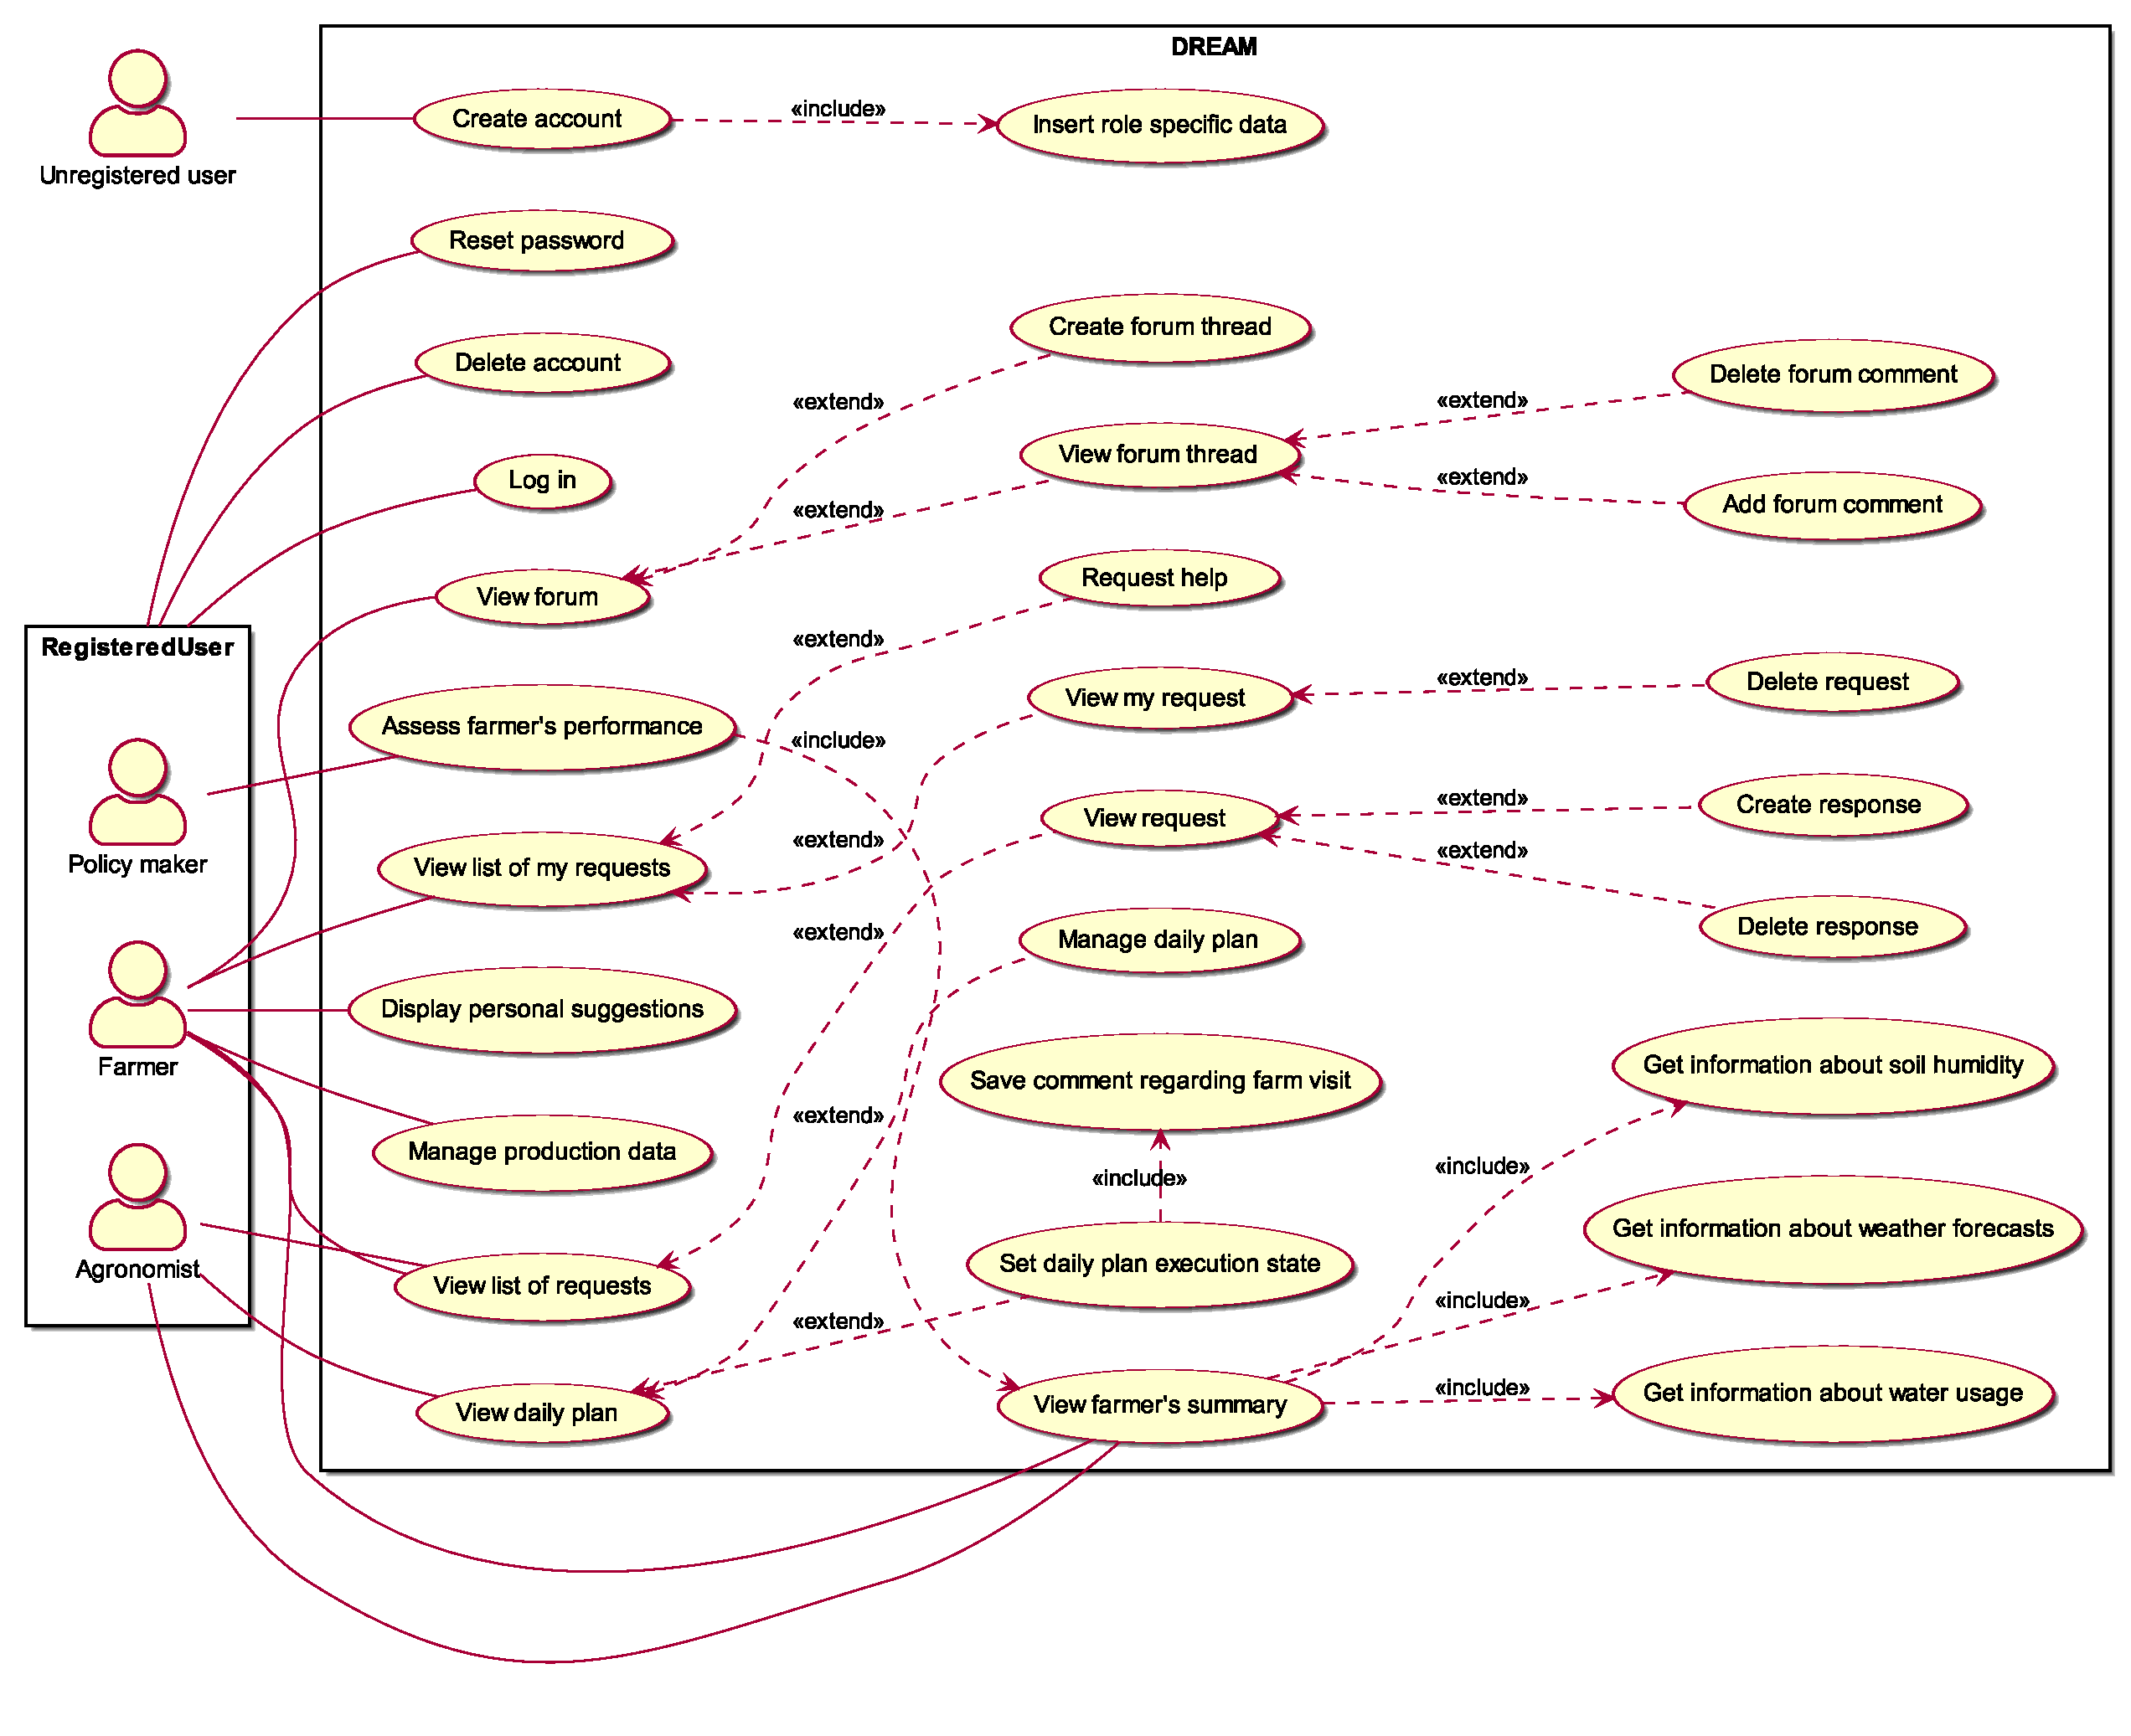
\includegraphics[width=0.96\textheight, keepaspectratio, origin=c, angle=90]{diagrams/use_case}
    \caption{Use case diagram}
    \label{fig:uc_diagram}
\end{figure}

% Definition of use case diagrams, 
% use cases and associated sequence/activity diagrams, 
% and mapping on requirements
\begin{table}[H]
    \centering
	\begin{tabular}{@{}p{0.25\linewidth} p{0.72\linewidth}@{}}
		\toprule
		\textbf{Name}               & Receive request notification\\
		\midrule
		\textbf{Id}                 & TODO\\
		\midrule
		\textbf{Actors}             & Agronomist, Farmer\\
		\midrule
		
		\textbf{Entry conditions}   & \begin{itemize}[leftmargin=.4cm,noitemsep,topsep=0pt,before=\vspace{-3mm},after=\vspace{-4mm}]
		    \item The farmer or the agronomist is already logged in to the application
		\end{itemize}\\
		\midrule
		
		\textbf{Flow of events}     & \begin{enumerate}[leftmargin=.4cm,noitemsep,topsep=0pt,before=\vspace{-3mm},after=\vspace{-4mm}]
		    \item The application indicates that unread notifications exist via a small number on the bell icon on the top bar.
		    \item The farmer or the agronomist clicks on the icon.
		    \item The application shows a list of unread notifications.
		    \item The farmer or the agronomist selects the unread notification to see.
		    \item The application shows details of the request.
		\end{enumerate}\\
		\midrule
		\textbf{Exit conditions}    & The application showed the notification contents. \\
		\midrule
		
		\textbf{Exceptions}         & \begin{itemize}[leftmargin=.4cm,noitemsep,topsep=0pt,before=\vspace{-3mm}]
		   \item The farmer or the agronomist cancels the operation during step 3.
		\end{itemize}
	    The system hides the list of unread notifications and shows only the main board screen.\\
		\bottomrule
	\end{tabular}
	\caption{Your caption here} 
\end{table}


\begin{center}
	\begin{tabular}{@{}p{0.25\linewidth} p{0.72\linewidth}@{}}
		\toprule
		\textbf{Name}               & Answer to a request\\
		\midrule
		\textbf{Id}                 & TODO\\
		\midrule
		\textbf{Actors}             & Agronomist, Farmer\\
		\midrule
		
		\textbf{Entry conditions}   & \begin{itemize}[leftmargin=.4cm,noitemsep,topsep=0pt,before=\vspace{-3mm},after=\vspace{-4mm}]
		    \item The farmer or the agronomist is already logged in to the application
		    \item The farmer or the agronomist has already read the notification
		\end{itemize}\\
		\midrule
		
		\textbf{Flow of events}     & \begin{enumerate}[leftmargin=.4cm,noitemsep,topsep=0pt,before=\vspace{-3mm},after=\vspace{-4mm}]
		    \item The farmer or the agronomist clicks \textit{Reply} under the request contents.
		    \item The farmer or the agronomist enters the contents of the reply message.
		    \item The farmer or the agronomist clicks the \textit{Send} button.
		    \item The application shows a message indicating successful sending of the message.
		\end{enumerate}\\
		\midrule
		\textbf{Exit conditions}    & The application notifies a farmer about the reply to the request. \\
		\midrule
		
		\textbf{Exceptions}         & \begin{itemize}[leftmargin=.4cm,noitemsep,topsep=0pt,before=\vspace{-3mm}]
		   \item The farmer or the agronomist cancels the operation during step 2.
		\end{itemize}
	    The system comes back to the screen with the list of notifications.\\
		\bottomrule
	\end{tabular}
\end{center}

\begin{center}
	\begin{tabular}{@{}p{0.25\linewidth} p{0.72\linewidth}@{}}
		\toprule
		\textbf{Name}               & Update daily plan\\
		\midrule
		\textbf{Id}                 & TODO\\
		\midrule
		\textbf{Actors}             & Agronomist\\
		\midrule
		
		\textbf{Entry conditions}   & \begin{itemize}[leftmargin=.4cm,noitemsep,topsep=0pt,before=\vspace{-3mm},after=\vspace{-4mm}]
		    \item The agronomist is already logged in to the application.
		\end{itemize}\\
		\midrule
		
		\textbf{Flow of events}     & \begin{enumerate}[leftmargin=.4cm,noitemsep,topsep=0pt,before=\vspace{-3mm},after=\vspace{-4mm}]
		    \item The agronomist selects the daily plan tab.
		    \item The agronomist selects a visit he wants to rearrange.
		    \item  The agronomist selects a new date for the visit selected in the previous step.
		    \item The agronomist confirms his choice.
		    \item The application shows a message indicating successful save of the visit's date.
		\end{enumerate}\\
		\midrule
		\textbf{Exit conditions}    & The new date of the visit is successfully saved in the application. \\
		\midrule
		
		\textbf{Exceptions}         & \begin{itemize}[leftmargin=.4cm,noitemsep,topsep=0pt,before=\vspace{-3mm}]
		   \item An agronomist cancels the operation during the step 3. \todo{add another exception if a visit can't be delayed anymore?}
		\end{itemize}
	    The system shows the daily plan tab view.\\
		\bottomrule
	\end{tabular}
\end{center}

\begin{center}
	\begin{tabular}{@{}p{0.25\linewidth} p{0.72\linewidth}@{}}
		\toprule
		\textbf{Name}               & Save farm visit information\\
		\midrule
		\textbf{Id}                 & TODO\\
		\midrule
		\textbf{Actors}             & Agronomist\\
		\midrule
		
		\textbf{Entry conditions}   & \begin{itemize}[leftmargin=.4cm,noitemsep,topsep=0pt,before=\vspace{-3mm},after=\vspace{-4mm}]
		    \item The agronomist is already logged in to the application.
		    \item The agronomist visited a farm.
		\end{itemize}\\
		\midrule
		
		\textbf{Flow of events}     & \begin{enumerate}[leftmargin=.4cm,noitemsep,topsep=0pt,before=\vspace{-3mm},after=\vspace{-4mm}]
		    \item The agronomist selects the daily plan tab.
		    \todo{is it a tab? do wee need to define it?}
		    \item The agronomist selects the visit to a farm he had already done. 
		    \item The agronomist enters information he collected during a farm visit to the text box.
		    \item The agronomist saves the information he entered.
		    \item The application shows a message indicating successful save of entered data.
		\end{enumerate}\\
		\midrule
		\textbf{Exit conditions}    & The information obtained during a visit to a farm is saved in the system. \\
		\midrule
		
		\textbf{Exceptions}         & \begin{itemize}[leftmargin=.4cm,noitemsep,topsep=0pt,before=\vspace{-3mm}]
		    \item An agronomist cancels the operation during the step 3.
		\end{itemize}
	    The system shows the daily plan tab view. 
	    \todo{the same as above}\\
		\bottomrule
	\end{tabular}
\end{center}

\subsection{Mapping on requirements}

\begin{center}
	\begin{tabular}{@{}p{0.06\linewidth} p{0.44\linewidth} p{0.44\linewidth}@{}}
		\toprule
		\textbf{Goal}   & \textbf{Domain assumption} & \textbf{Requirement} \\
		\midrule
		\autonum{G} & & \\
		\autonum{G} & & \\
		\autonum{G} & & \\
		\autonum{G} & & \\
		\bottomrule
	\end{tabular}
\end{center}


\section{Performance Requirements} \label{sec:performance_requirements}

Given that the system is intended for Telangana farmers, agronomists, and policymakers, it is fair to assume that it will be utilized by about 30 000 people. Therefore, the following performance requirements, which were formulated taking into consideration the best practices \cite{performance_requirements}, should be met.

\subsection{Response Time}

\begin{itemize}
    \item During peak hours, the average response time should be 2 seconds.
    \item During peak hours, 99\% of all response times must be shorter than 3 seconds.
    \item In each 10-minute period commencing on the hour, the average response time must be 2 seconds or less.
    \item 95\% percent of all response times must be shorter than 2 seconds.
\end{itemize}
 
\subsection{Workload}

\begin{itemize}
    \item The system must be capable of processing 20 transactions per second.
    \item The system must have no more than one hour of downtime every three months.
\end{itemize}

\subsection{Scalability}

\begin{itemize}
    \item The system must be able to sustain a 5\% yearly growth in new users.
    \item The system must be able to sustain a 10\% yearly increase in the number of transactions per second.
    \item The system shall be able to extend its connections to new external systems providing relevant data as their number may arise.
\end{itemize}

\subsection{Platform}

DREAM has to be housed on a platform that meets the following criteria:

\begin{itemize}
    \item Operating system: Windows 10 or Windows 11.    
    \item \textit{.NET 6.0} development platform installed.
    \item \textit{PostgreSQL} object-relational database system.
    \item CPU: 1.4 GHz 64-bit processor compatible with x64 instruction set.
    \item Memory: Minimum 8 GB of RAM. 
    \item Hard drive space: minimum of 20 GB of space.
    \item Network adapter: an Ethernet adapter capable of at least 1 gigabit per second throughput.
\end{itemize}

\section{Design Constraints}

This section describes the constraints of a design. These include uncontrolled limitations that are self-imposed in order to enhance the design.

\subsection{Standards compliance}

The system will collect data \todo{so, are we collecting the data or just reading?} from external systems and sensors, as well as data entered by users during registration and application use, such as production data, agronomist's daily plan, farmer's summary, and notes. The data will be used exclusively for system purposes and will be treated discreetly in accordance with the General Data Protection Regulation \cite{GDPR} and IS 17428.1 \cite{india_privacy_doc} guidelines. In particular, no information relating to a specific person will be made public as a result of the statistical analyses undertaken.

\subsection{Hardware limitations}

The following are the hardware constraints that the end user must meet in order to use the system.

\begin{itemize}
    \item Processor: 1.9 GHz x86- or x64-bit dual-core processor.
    \item Memory: 2 GB of RAM.
    \item Network: wired or wireless connection with bandwidth greater than 40 KBps (320 kbps) and latency under 200 ms.
    \item Web browser: Google Chrome, Firefox, Safari, Microsoft Edge, or Opera running on Windows, macOS, Linux, or mobile operating systems including Android and iOS, with \textit{JavaScript} enabled.
\end{itemize}

\subsection{Any other constraints}

DREAM will employ stateless protocols to enable components to be handled and changed without impacting the overall system. Additionally, the system will catalog, retrieve and run queries on all the relevant data using a relational database.

\section{Software System Attributes}

The system's characteristics that facilitate the measurement of its performance are presented in this section.

\subsection{Reliability}

The mean time between failures shall be equal to 120 hours, which means that in the worst case scenario it may break once every 5 days. Furthermore, the system shall be fault-tolerant, with its architecture prepared for any potential damage to system components by having replicas ready to be substituted. In order to recover from eventual data losses, redundancy should be considered for the system's database implementation.

\subsection{Availability}

As mentioned in the section \ref{sec:performance_requirements}, the system shall have no more than one hour of downtime every three months, thus, shall be highly available. In case of any planned maintenance works, all the users should be notified at least 48 hours in advance.

\subsection{Security}

The system shall implement role-based access control, which is a method of restricting system access to authorized users and granting permissions based on the user's role. It is accomplished through the use of both authentication and authorization implemented in the backend. The former is based on verifying the identity of a user, which can be an agronomist, a farmer, or a policy maker, during the log in phase. The latter, on the other hand, validates the logged-in user's permissions to perform an action (for example, visualizing an agronomist's daily plan) before actually carrying it out.

\subsection{Maintainability}

The system shall be written in a widely known programming language, which would ensure a high level of maintainability and a relatively simple induction for potential new members of the development team. Following that, it should be divided into modularized components to ease replacements and fixes in the event of a failure. The system's backend must be capable of supporting maintenance works on a copy, which will subsequently be deployed after being tested on pre-defined test suites, in order to ensure no downtime for the core functionalities.

Both the testing scenarios and the tests themselves should be defined. This contains both end-to-end testing and basic unit tests. The code coverage should then be monitored and controlled. In the event of a system failure, thorough crash reports must be sent to the developers.

Maintenance pauses will be arranged on occasion throughout the night, when user traffic is at its lowest.

\subsection{Portability}

DREAM will be offered as a web application, making it available on the vast majority of current web browsers, including desktop and mobile machines. Because of this approach, the system will be usable on a wide range of devices. User interface adjustments shall be made to make the application user-friendly on all the environments.
